\documentclass[12pt,t]{beamer}
% \documentclass[t]{beamer}
\usepackage[utf8]{inputenc}
\usepackage[catalan]{babel}
\usepackage{verbatim}
\usepackage{hyperref}
\usepackage{amsfonts,amssymb,amsmath,amsthm, wasysym, multirow}
\usepackage{listings}
\usepackage[T1]{fontenc}        
\usepackage{pgf}
\usepackage{epsdice}
\usepackage{pgfpages}
\usepackage{tikz}
%\usetikzlibrary{arrows,shapes,plotmarks,backgrounds,trees,positioning}
%\usetikzlibrary{decorations.pathmorphing,calc,snakes}
%\usepackage{marvosym}
%
\usetheme[hideothersubsections,left]{Marburg}
\usecolortheme{sidebartab}
\useinnertheme[shadow]{rounded}
% \useoutertheme[footline=empty,subsection=true,compress]{infolines}
% \useoutertheme[footline=empty,subsection=true,compress]{miniframes}
% \usefonttheme{serif}

\setbeamertemplate{caption}[numbered]
\setbeamertemplate{navigation symbols}{}


\newcommand{\red}[1]{\textcolor{red}{#1}}
\newcommand{\green}[1]{\textcolor{green}{#1}}
\newcommand{\blue}[1]{\textcolor{blue}{#1}}
\newcommand{\gray}[1]{\textcolor{gray}{#1}}
\renewcommand{\emph}[1]{{\color{red}#1}}

\setbeamertemplate{frametitle}
{\begin{centering}
\medskip
\color{blue}
\textbf{\insertframetitle}
\medskip
\end{centering}
}
\usecolortheme{rose}
\usecolortheme{dolphin}
\mode<presentation>


\newcommand{\CC}{\mathbb{C}}
\newcommand{\RR}{\mathbb{R}}
\newcommand{\ZZ}{\mathbb{Z}}
\newcommand{\NN}{\mathbb{N}}
\newcommand{\KK}{\mathbb{K}}
\newcommand{\MM}{\mathcal{M}}
%\newcommand{\dbinom}{\displaystyle\binom}

\newcommand{\limn}{{\displaystyle \lim_{n\to\infty}}}
\renewcommand{\leq}{\leqslant}
\renewcommand{\geq}{\geqslant}
\def\tendeix{{\displaystyle\mathop{\longrightarrow}_{\scriptscriptstyle
n\to\infty}}}

\newcommand{\matriu}[1]{\left(\begin{matrix} #1 \end{matrix}\right)}

% \newcommand{\qed}{\hbox{}\nobreak\hfill\vrule width 1.4mm height 1.4mm depth 0mm
%     \par \goodbreak \smallskip}
%
% %
\theoremstyle{plain}
\newtheorem{teorema}{Teorema}
\newtheorem{prop}{Proposició}
\newtheorem{cor}{Coro\l.lari}
\theoremstyle{definition}
\newtheorem{exemple}{Exemple}
\newtheorem{defin}{Definició}
\newtheorem{obs}{Observació}

\newcounter{seccions}
\newcommand{\seccio}[1]{\addtocounter{seccions}{1}
\medskip\par\noindent\emph{\theseccions.
#1}\smallskip\par }

\newcommand{\EM}{\Omega}
\newcommand{\PP}{\mathcal{P}}

\title[\red{Matemàtiques III}]{}
\author[]{}
\date{}



\begin{document}
\beamertemplatedotitem

\lstset{backgroundcolor=\color{green!50}}
\lstset{breaklines=true}
\lstset{basicstyle=\ttfamily}


\begin{frame}
\vfill
\begin{center}
\gray{\LARGE Regressió lineal}
\end{center}
\vfill
\end{frame}



\section{Regressió lineal simple}
\subsection{Regressió lineal}

\begin{frame}
\frametitle{Regressió lineal}

La taula següent dóna l'alçada mitjana (en cm) dels nins a determinades edats (en anys):
\begin{center}
\begin{tabular}{c|ccccccc}
\hline
edat & 1 & 3 & 5 & 7 & 9 & 11 & 13\\
\hline
alçada & 75 & 92 & 108 & 121 & 130 & 142 & 155\\
\hline
\end{tabular}
\end{center}
A la lliçó 2 de R-I calculàvem amb R la millor relació lineal
$$
\mbox{alçada}\approx b_0+b_1\cdot\mbox{edat}
$$ 
\end{frame}



\begin{frame}[fragile]
\frametitle{Regressió lineal}
\vspace*{-2ex}

\begin{verbatim}
> edat=c(1,3,5,7,9,11,13)
> alçada=c(75,92,108,121,130,142,155)
> plot(edat,alçada)
> abline(lm(alçada~edat))
\end{verbatim}
\vspace*{-4ex}

\begin{center}
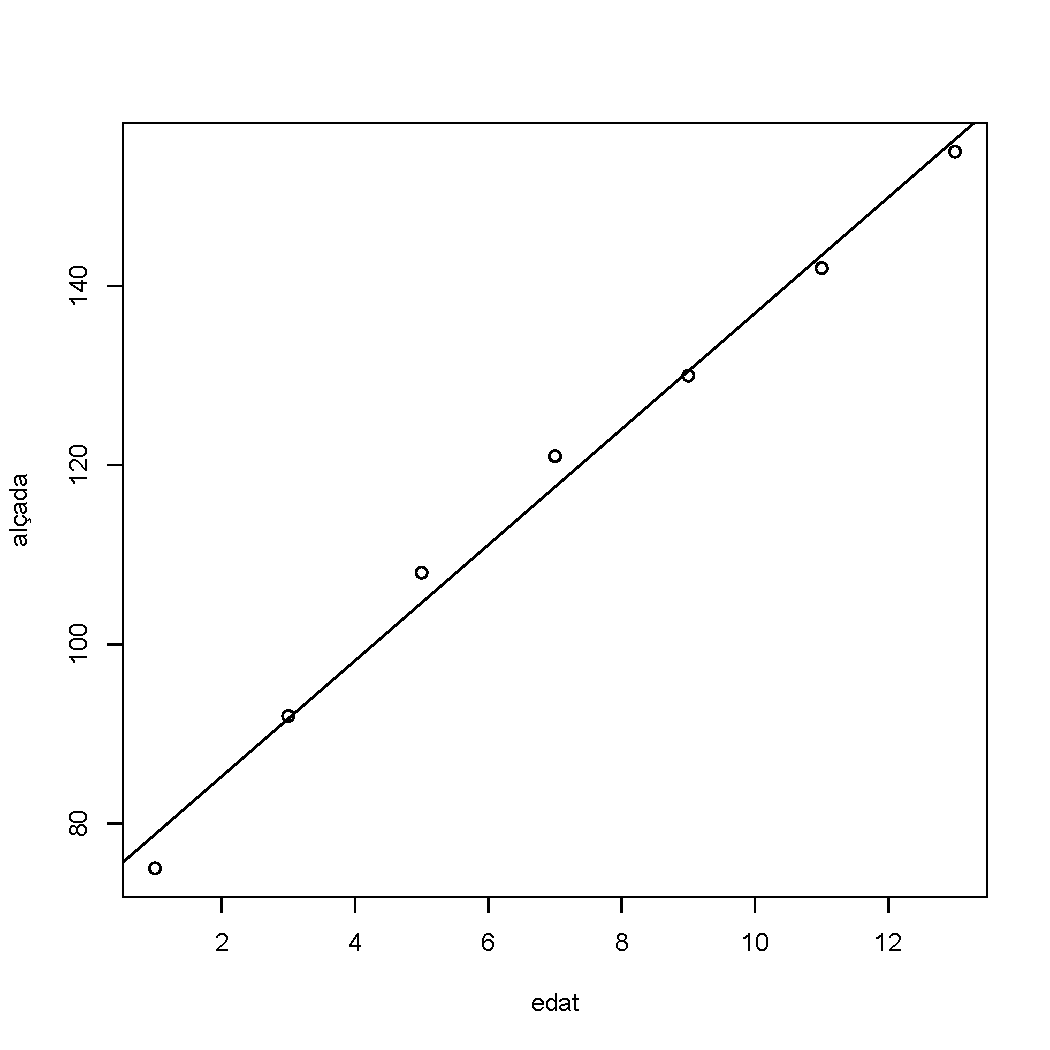
\includegraphics[width=0.7\linewidth]{ed-al2.pdf}
\end{center}
\end{frame}

\begin{frame}
\frametitle{Regressió lineal simple}
Tenim parelles d'observacions de dues variables $X,Y$:
$$
(x_i,y_i)_{i=1,2,\ldots,n}
$$
i volem estudiar com depèn el valor de $Y$ del de $X$:
\medskip

\begin{itemize}
\item La variable aleatòria $Y$ és la variable \emph{dependent} o \emph{de resposta}

\item La variable (no necessàriament aleatòria) $X$ és la variable \emph{de control},
\emph{independent} o \emph{de regressió}
\end{itemize}
\bigskip

Volem trobar la millor relació funcional que  expliqui la variable $Y$ conegudes les observacions de la
variable $X$. Per ara, cercam una \emph{relació lineal} que expliqui $Y$ en funció de $X$.
\end{frame}

\begin{frame}
\frametitle{Regressió lineal simple}

Suposam que 
$$
\mu_{Y|x}=\beta_0+\beta_1 x
$$
on $\mu_{Y|x}$ és el valor esperat de $Y$ quan $X$ val $x$, i $\beta_0$
(\emph{terme independent}) i $\beta_1$ (\emph{pendent}) són dos
paràmetres que volem estimar
\medskip

Amb una mostra $(x_i,y_i)_{i=1,2,\ldots,n}$, calcularem estimacions $b_0$ i $b_1$ de
$\beta_0$ i de $\beta_1$
\medskip

Això ens donarà la \emph{recta de regressió} per a la nostra mostra:
$$
\widehat{y}=b_0+b_1 x
$$
que donat un valor $x_0$ de $X$ ens estimarà el valor $\widehat{y}_0=b_0+b_1 x_0$ de $Y$ sobre el mateix individu
\end{frame}

\begin{frame}
\frametitle{Regressió lineal simple}

El model anterior el reescrivim com a
$$
\begin{array}{rl}
Y|x &=\mu_{Y|x}+ E_x\\
&=\beta_0+\beta_1 x+ E_x,
\end{array}
$$
on
\begin{itemize}
\item $Y|x$ és la variable aleatòria ``valor de $Y$ quan $X$ val $x$''
\medskip

\item $E_x$ és la variable aleatòria \emph{error} o \emph{residu}, que dóna la diferència entre el valor de $Y$ i el valor ``esperat'' $\mu_{Y|x}$, és a dir, $\beta_0+\beta_1 x$
\medskip

\item Com que suposam que $\mu_{Y|x}=\beta_0+\beta_1 x$, suposam que $\mu_{E_x}=0$ per a cada $x$
\end{itemize}

\end{frame}

\subsection{Mínims quadrats}

\begin{frame}
\frametitle{Mínims quadrats}

Per a cada observació $(x_i,y_i)$, tendrem
$$
y_i=\beta_0+\beta_1 x_i+ \varepsilon_i\Rightarrow \varepsilon_i=y_i-(\beta_0+\beta_1 x_i)
$$
\smallskip

Diguem l'\emph{error quadràtic teòric} d'aquest model a
$$
\red{SS_\varepsilon}=\sum_{i=1}^n \varepsilon_i^2=\sum_{i=1}^n (y_i-\beta_0-\beta_1 x_i)^2
$$
A la \emph{regressió lineal per mínims quadrats}, els estimadors $b_0$ i $b_1$ de $\beta_0$ i $\beta_1$ que cercam són els valors de ``les incògnites''  $\beta_0$ i $\beta_1$ que minimitzen aquest  $SS_\varepsilon$
\end{frame}

\begin{frame}
\frametitle{Mínims quadrats}
Anem a minimitzar $SS_\varepsilon$. El mínim $(b_0,b_1)$ de
$$
SS_\varepsilon=\sum_{i=1}^n (y_i-\beta_0-\beta_1 x_i)^2
$$
anu\l.larà les derivades respecte de $\beta_0$ i $\beta_1$.
\medskip

Derivem:
$$
\begin{array}{ll}
\dfrac{\partial SS_\varepsilon}{\partial \beta_0}=&-2\sum\limits_{i=1}^n (y_i -\beta_0-\beta_1 x_i)\\[2ex]
\dfrac{\partial SS_\varepsilon}{\partial \beta_1}=&-2\sum\limits_{i=1}^n (y_i -\beta_0-\beta_1 x_i) x_i 
\end{array}
$$
\end{frame}

\begin{frame}
\frametitle{Mínims quadrats}
El $(b_0,b_1)$ que cercam satisfà
$$
\begin{array}{l}
2\sum\limits_{i=1}^n (y_i -b_0-b_1 x_i)=0\\[2ex]
2\sum\limits_{i=1}^n (y_i -b_0-b_1 x_i) x_i =0
\end{array}
$$
Reescrivim:
$$
\begin{array}{rl}
n b_0 + \Big(\sum\limits_{i=1}^n x_i\Big) b_1 & =\sum\limits_{i=1}^n y_i\\[1ex]
\Big(\sum\limits_{i=1}^n x_i\Big) b_0 + \Big(\sum\limits_{i=1}^n x_i^2\Big) b_1 &=\sum\limits_{i=1}^n x_iy_i
\end{array}
$$
\end{frame}

\begin{frame}
\frametitle{Mínims quadrats}
Les solucions són
$$
\begin{array}{rl}
b_1& \displaystyle=\frac{n \sum\limits_{i=1}^n x_i y_i-\sum\limits_{i=1}^n x_i\sum\limits_{i=1}^n y_i} {n\sum\limits_{i=1}^n
x_i^2-(\sum\limits_{i=1}^n x_i)^2}\\[6ex]
b_0& \displaystyle=\frac{\sum\limits_{i=1}^n y_i -b_1 \sum\limits_{i=1}^n x_i}{n}
\end{array}
$$
i  donen el mínim de $SS_\varepsilon$
\end{frame}

\begin{frame}
\frametitle{Mínims quadrats}
Considerem les mitjanes
$$
\overline{x}=\frac{1}{n}\sum\limits_{i=1}^n x_i,
\quad \overline{y}=\frac{1}{n} \sum\limits_{i=1}^n y_i
$$
i les variàncies i covariància 
$$
\begin{array}{rl}
s_x^2 &\displaystyle =\frac{1}{n}\sum_{i=1}^n (x_i-\overline{x})^2 =\frac{1}{n}\Big(\sum_{i=1}^n x_i^2\Big) -\overline{x}^2\\[2ex]
s_y^2 &\displaystyle =\frac{1}{n}\sum_{i=1}^n (y_i-\overline{y})^2 =\frac{1}{n}\Big(\sum_{i=1}^n y_i^2\Big) -\overline{y}^2\\[2ex]
s_{xy} &\displaystyle =\frac{1}{n}\sum_{i=1}^n (x_i-\overline{x}) (y_i-\overline{y}) =\frac{1}{n}\Big(\sum_{i=1}^n x_i y_i\Big)-\overline{x}\cdot\overline{y}
\end{array}
$$
\end{frame}

\begin{frame}
\frametitle{Mínims quadrats}
Els valors de $b_0$ i $b_1$ trobats abans es poden reescriure de la forma següent:

\begin{teorema}
Els estimadors $b_0$ i $b_1$ per mínims quadrats de $\beta_0$ i $\beta_1$ són
$$
b_1 =\frac{s_{xy}}{s_x^2},\quad b_0 = \overline{y}-b_1 \overline{x}.
$$
\end{teorema}
Escriurem
$$
\widehat{y}=b_0+b_1x
$$
Direm a $\widehat{y}$ el \emph{valor estimat} de $Y$ quan $X=x$
\medskip

Per a cada observació $(x_i,y_i)$, direm l'\emph{error} a 
$$
\red{e_i}=y_i-\widehat{y}_i={y}_i-b_0-b_1x_i
$$
\end{frame}

\begin{frame}[fragile]
\frametitle{Exemple 1}
Volíem calcular la recta de regressió per mínims quadrats de
\begin{center}
\begin{tabular}{c|ccccccc}
\hline
edat ($x$) & 1 & 3 & 5 & 7 & 9 & 11 & 13\\
\hline
alçada ($y$) & 75 & 92 & 108 & 121 & 130 & 142 & 155\\
\hline
\end{tabular}
\end{center}
\begin{verbatim}
> x=c(1,3,5,7,9,11,13)
> y=c(75,92,108,121,130,142,155)
> x.b=mean(x)
> y.b=mean(y)
> s2.x=var(x)*6/7
> s2.y=var(y)*6/7
> s.xy=cov(x,y)*6/7
> round(c(x.b,y.b,s2.x,s2.y,s.xy),3)
[1]   7.000 117.571  16.000 674.531 103.429
\end{verbatim}
\end{frame}

\begin{frame}[fragile]
\frametitle{Exemple 1}
\vspace*{-2ex}

\begin{center}
\begin{tabular}{cccccccc}
$\overline{x}$ &  $\overline{y}$ & $s_x^2$ & $s_y^2$ & $s_{xy}$\\ \hline
7.000 & 117.571 & 16 & 674.531 & 103.429
\end{tabular}
\end{center}
$$
\begin{array}{l}
\displaystyle b_1 =\frac{s_{xy}}{s_x^2}=\frac{103.429}{16}=6.4643\\[2ex]
\displaystyle b_0 = \overline{y}-b_1 \overline{x} =117.571-6.4643\cdot 7=72.3209
\end{array}
$$
Obtenim
$$
\widehat{y}=72.3209+6.4643x
$$
\medskip

\begin{verbatim}
> lm(y~x)$coefficients
(Intercept)           x 
  72.321429    6.464286 
\end{verbatim}
\end{frame}

\begin{frame}[fragile]
\frametitle{Alerta!}

Els càlculs involucrats en la regressió lineal són molt poc robusts: els arrodoniments
poden influir molt en el resultat final
\bigskip

A la Wikipedia (\url{http://en.wikipedia.org/wiki/Simple_linear_regression}) hi trobareu un exemple detallat d'una regressió de pes en funció d'alçada. Calculada en metres dóna:
$$
\widehat{y}=61.272x-39.062
$$
Si es passen les alçades a polzades, s'arrodoneixen, es calcula la recta de regressió, i es torna a passar  el resultat a metres, dóna
$$
\widehat{y}=61.675x-39.746
$$




\end{frame}



\begin{frame}
\frametitle{Exemple 2}
En un experiment on es volia estudiar l'associació entre consum de sal i pressió arterial, a alguns individus se'ls assignà aleatòriament una quantitat diària constant de sal en la seva dieta, i al cap d'un mes se'ls mesurà la tensió mitjana. Alguns resultats varen ser els següents
\begin{center}
\begin{tabular}{cc}
$X$ (sal, en g) 	& $Y$ (Pressió, en mm de Hg)\\ \hline
1.8 &	100\\
2.2 &	98\\
3.5 &	110\\
4.0 &	110\\
4.3 &	112\\
5.0 &	120\\
\end{tabular}
\end{center}
Trobau la recta de regressió lineal per mínims quadrats de $Y$ en funció de $X$

\end{frame}

\begin{frame}
\frametitle{Exemple 2}

\begin{center}
\begin{tabular}{ccccc}
$\overline{x}$ &  $\overline{y}$ & $s_x^2$ & $s_y^2$ & $s_{xy}$\\ \hline
3.467 & 108.333 & 1.2856 &55.2222 & 8.1444
\end{tabular}
\end{center}
\bigskip

$$
\begin{array}{l}
\displaystyle b_1 =\vphantom{\frac{s_{xy}}{s_x^2}}\hphantom{\overline{y}-b_1 \overline{x} = 86.371}\\[2ex]
\displaystyle b_0 =\hphantom{\overline{y}-b_1 \overline{x} = 86.371}
\end{array}
$$
\bigskip

Obtenim la recta
$$
\widehat{y}= \hphantom{86.371+6.335x}
$$

\end{frame}


\begin{frame}
\frametitle{Exemple 2}

\begin{center}
\begin{tabular}{ccccc}
$\overline{x}$ &  $\overline{y}$ & $s_x^2$ & $s_y^2$ & $s_{xy}$\\ \hline
3.467 & 108.333 & 1.2856 &55.2222 & 8.1444
\end{tabular}
\end{center}
\bigskip

$$
\begin{array}{l}
\displaystyle b_1 =\frac{s_{xy}}{s_x^2}=6.335\\[2ex]
\displaystyle b_0 = \overline{y}-b_1 \overline{x} = 86.371
\end{array}
$$
\bigskip

Obtenim la recta
$$
\widehat{y}= 86.371+6.335x
$$

\end{frame}


\begin{frame}[fragile]
\frametitle{Exemple 2}
Com podem comprovar, amb R dóna ``el mateix''
\begin{verbatim}
> sal=c(1.8,2.2,3.5,4,4.3,5)
> ten=c(100,98,110,110,112,120)
> lm(ten~sal)$coefficients
(Intercept)         sal 
   86.37079     6.33535 
\end{verbatim}
\end{frame}



\begin{frame}
\frametitle{Propietats}

\begin{itemize}
\item La recta de regressió passa pel vector mitjà
$(\overline{x},\overline{y})$:
$$
b_0+b_1 \overline{x}=\overline{y}
$$

\item La mitjana dels valors estimats és igual a la mitjana dels
observats:
$$
\red{\overline{\widehat{y}}=}\frac{1}{n}\sum_{i=1}^n\widehat{y}_i
=\frac{1}{n}\sum_{i=1}^n(b_0+b_1x_i)=
b_0+b_1 \overline{x}=\red{\overline{y}}
$$

\item Els errors $(e_i)_{i=1,\ldots,n}$ tenen mitjana 0:
$$
\hspace*{-0.7cm}\red{\overline{e}
=}\frac{1}{n}\sum_{i=1}^n e_i
=\frac{1}{n}\sum_{i=1}^n (y_i-b_0-b_1x)
=\frac{1}{n}\sum_{i=1}^n (y_i-\widehat{y}_i)
=\red{0}
$$
\end{itemize}
\end{frame}



\begin{frame}
\frametitle{Propietats}
Direm \emph{suma de quadrats dels errors} a
$$
\red{SS_E}=\sum_{i=1}^{n} e^2_i
$$
\medskip

Els errors $(e_i)_{i=1,\ldots,n}$ tenen variància
$$
\red{s_e^2=}\frac{1}{n}\Big(\sum_{i=1}^{n}
e^2_i\Big)-\overline{e}^2=\frac{SS_E}{n}-0=\red{\frac{SS_E}{n}}
$$

\end{frame}


\begin{frame}
\frametitle{Propietats}

\begin{teorema}
Si les variables aleatòries error $E_{x_i}$ tenen totes mitjana 0 i la mateixa variància $\sigma^2_E$ i, dues a dues, tenen covariància 0, aleshores

\begin{itemize}
\item $b_0$ i $b_1$ són els estimadors lineals no esbiaixats òptims (més eficients) de $\beta_0$ i $\beta_1$
\medskip

\item Un estimador no esbiaixat de $\sigma_E^2$ és
$$
S^2=\frac{SS_E}{n-2}
$$
\end{itemize}
\end{teorema}
\end{frame}



\begin{frame}
\frametitle{Propietats}

\begin{teorema}
Si \emph{a més} les variables aleatòries error $E_{x_i}$ són normals, aleshores
 $b_0$ i $b_1$ són els estimadors màxim versemblants de $\beta_0$ i $\beta_1$ (i no esbiaixats)
 \end{teorema}
\end{frame}





\begin{frame}[fragile]
\frametitle{Exemple 1}
Si suposam que al nostre exemple d'edats i alçades els errors tenen la mateixa variància i són incorrelats, podem estimar aquesta variància:
\begin{verbatim}
> x=c(1,3,5,7,9,11,13)
> y=c(75,92,108,121,130,142,155)
> y.cap=72.321+6.464*x
> errors=y-y.cap
> SSE=sum(errors^2)
> S2=SSE/(length(x)-2)
> S2
[1] 8.314296
\end{verbatim}
Tenim que $S^2=8.3143$, i estimam que $\sigma_E^2$ val això
\end{frame}

\begin{frame}[fragile]
\frametitle{Exemple 2}
Si suposam que al nostre exemple de sal i tensió arterial els errors  tenen la mateixa variància i són incorrelats, podem estimar aquesta variància:
\begin{verbatim}
> sal=c(1.8,2.2,3.5,4,4.3,5)
> ten=c(100,98,110,110,112,120)
> ten.cap=86.371+6.335*sal
> errors.ten=ten-ten.cap
> SSE=sum(errors.ten^2)
> S2=SSE/(length(sal)-2)
> S2
[1] 5.436475
\end{verbatim}
Tenim que $S^2=5.4365$, i estimam que $\sigma_E^2$ val això
\end{frame}





\begin{frame}
\frametitle{Això és tot?}
Hem estimat els coeficients $\beta_0$ i $\beta_1$ i la variable $Y|x$, per a cada $x$,  al model
$$
\mu_{Y|x}=\beta_0+\beta_1 x
$$
però ens pot interessar més:
\medskip

\begin{itemize}
\item Com és de significativa l'estimació obtinguda?
\medskip

\item Error estàndard d'aquests estimadors
\medskip

\item Intervals de confiança 
\end{itemize}
\end{frame}




\begin{frame}[fragile]
\frametitle{Amb R obtenim molt més\ldots}
\footnotesize \begin{verbatim}
> summary(lm(alçada~edat))
...
Coefficients:
            Estimate Std. Error t value Pr(>|t|)    
(Intercept)  72.3214     2.1966   32.92 4.86e-07 ***
edat          6.4643     0.2725   23.73 2.48e-06 ***
---
Signif. codes:  0 ‘***’ 0.001 ‘**’ 0.01 ‘*’ 0.05
   ‘.’ 0.1 ‘ ’ 1 

Residual standard error: 2.883 on 5 degrees of freedom
Multiple R-squared: 0.9912,	Adjusted R-squared: 0.9894 
F-statistic: 562.9 on 1 and 5 DF,  p-value: 2.477e-06 
\end{verbatim}
\end{frame}


\subsection{Coeficient de determinació}
\begin{frame}[fragile]
\frametitle{Com és de significativa la regressió?}

Entenem que la recta $\widehat{y}=b_0+b_1x$ és una bona aproximació de $y$ com a funció lineal de $x$ quan 
aquesta recta explica
molta part de la variabilitat de $y$\bigskip

Es quantifica amb el \emph{coeficient de determinació $R^2$}
\begin{verbatim}
> summary(lm(alçada~edat))$r.squared
[1] 0.9911957
\end{verbatim}

\end{frame}

\begin{frame}
\frametitle{Sumes de quadrats}
Siguin:
\begin{itemize}
\item $\red{SS_T} =\sum\limits_{i=1}^n(y_i-\overline{y})^2$: suma total de quadrats
$$
SS_T=n\cdot s_y^2
$$

\item $\red{SS_R}=\sum\limits_{i=1}^n(\widehat{y}_i-\overline{y})^2$: suma de quadrats de la regressió 
$$
SS_R=n\cdot s_{\widehat{y}}^2
$$

\item $\red{SS_E}=\sum\limits_{i=1}^n(y_i-\widehat{y}_i)^2$: suma de quadrats dels errors
$$
SS_E=n\cdot s_e^2
$$
\end{itemize}

\end{frame}

\begin{frame}
\frametitle{Sumes de quadrats}

\begin{teorema}
En una regressió lineal pel mètode de mínims quadrats, es té que
$$
SS_T=SS_R+SS_E
$$
o equivalentment,
$$
s^2_y=s^2_{\widehat{y}}+s^2_e
$$
\end{teorema}

\end{frame}
%
%\begin{frame}[fragile]
%\frametitle{Exemple 1}
%\vspace*{-2ex}
%
%\begin{verbatim}
%> x=c(1,3,5,7,9,11,13)
%> y=c(75,92,108,121,130,142,155)
%> y.cap=72.321+6.464*seq(1,13,2)
%> errors=y-y.cap
%> SST=sum((y-mean(y))^2)
%> SSR=sum((y.cap-mean(y))^2)
%> SSE=sum((y-y.cap)^2)
%> c(SST,SSR,SSE)
%[1] 4721.71429 4679.72919   41.57148
%> SSR+SSE
%[1] 4721.301
%\end{verbatim}
%\end{frame}
%
%
%\begin{frame}[fragile]
%\frametitle{Exemple 1}
%\vspace*{-2ex}
%
%
%\begin{verbatim}
%> x=c(1,3,5,7,9,11,13)
%> y=c(75,92,108,121,130,142,155)
%> lm(y~x)$coefficients
%(Intercept)           x 
%  72.321429    6.464286 
%> y.cap=lm(y~x)$coefficients[1]+lm(y~x)$coefficients[2]*seq(1,13,2)
%> errors=y-y.cap
%> SST=sum((y-mean(y))^2)
%> SSR=sum((y.cap-mean(y))^2)
%> SSE=sum(errors^2)
%> c(SST,SSR,SSE)
%[1] 4721.71429 4680.14286   41.57143
%> SSR+SSE
%[1] 4721.714
%\end{verbatim}
%\end{frame}
%

\begin{frame}
\frametitle{El coeficient de determinació $R^2$}
El \emph{coeficient de determinació} d'una regressió lineal és
$$
\red{R^2}=\frac{SS_R}{SS_T}=\frac{s_{\widehat{y}}^2}{s_y^2}
$$
Per tant, $R^2$ és la fracció de la variabilitat de $y$ que queda explicada per la variabilitat de $\widehat{y}$
\bigskip


Si la regressió lineal és per mínims quadrats,
$$
R^2=\frac{SS_T-SS_E}{SS_T}=1-\frac{SS_E}{SS_T}=1-\frac{s_e^2}{s_y^2}
$$
\end{frame}


\begin{frame}
\frametitle{El coeficient de determinació $R^2$}
A més, \emph{$R^2=r_{xy}^2$}, el coeficient de correlació al quadrat
$$
\begin{array}{rl}
R^2 & \displaystyle =\frac{SS_R}{SS_T}=\frac{\sum\limits_{i=1}^n(b_1x_i+b_0-\overline{y})^2}{ns_y^2}\\[2ex] 
& \displaystyle =\frac{\sum\limits_{i=1}^n(\dfrac{s_{xy}}{s_x^2}x_i-\dfrac{s_{xy}}{s_x^2}\overline{x})^2}{ns_y^2}\\[2ex] 
& \displaystyle =\frac{\dfrac{s_{xy}^2}{s_x^4}\sum\limits_{i=1}^n(x_i-\overline{x})^2}{ns_y^2}\\[2ex] & \displaystyle =\dfrac{s_{xy}^2}{s_x^4}\cdot \frac{s_x^2}{s_y^2}=\frac{s_{xy}^2}{s_x^2\cdot s_y^2}=r_{xy}^2
\end{array}
$$
\end{frame}

%
%\begin{frame}
%\frametitle{El coeficient de determinació $R^2$}
%A més:
%
%\begin{itemize}
%\item Un estimador no esbiaixat de $\sigma_E^2$ (la variància de la variable aleatòria Error $E$) és
%$$
%S^2=\frac{SS_E}{n-2}
%$$
%\end{itemize}
%\end{frame}

\begin{frame}[fragile]
\frametitle{Exemple 1}
\vspace*{-2ex}

\begin{verbatim}
> x=c(1,3,5,7,9,11,13)
> y=c(75,92,108,121,130,142,155)
> y.cap=72.321+6.464*x
> SST=sum((y-mean(y))^2)
> SSR=sum((y.cap-mean(y))^2)
> SSE=sum((y-y.cap)^2)
> round(c(SST,SSR,SSE),3)
[1] 4721.714 4679.729  41.571
\end{verbatim}
$$
R^2=\frac{4679.729}{4721.714}=0.9912
$$
\begin{verbatim}
> cor(x,y)^2
[1] 0.9911957
\end{verbatim}
\end{frame}

\begin{frame}[fragile]
\frametitle{Exemple 2}
\vspace*{-3ex}

\small \begin{verbatim}
> sal=c(1.8,2.2,3.5,4,4.3,5)
> ten=c(100,98,110,110,112,120)
> ten.cap=86.371+6.335*sal
> SST=sum((ten-mean(ten))^2)
> SSR=sum((ten.cap-mean(ten))^2)
> SSE=sum((ten-ten.cap)^2)
> round(c(SST,SSR,SSE),3)
[1] 331.333 309.553  21.746
\end{verbatim}
$$
R^2=\pause\frac{SS_R}{SS_T}=\frac{309.553}{331.333}=0.934
$$
\begin{verbatim}
> cor(sal,ten)^2
[1] 0.9343685
> summary(lm(ten~sal))$r.squared
[1] 0.9343685
\end{verbatim}
\end{frame}

\begin{frame}[fragile]{El valor de $R^2$ no és suficient!}
No és possible valorar la bondat del model només basant-se amb el valor de $R^2$. Vegem quatre conjunts de parells $(x_i,y_i)$, generats específicament amb aquest objectiu, continguts en el data frame \texttt{anscombe} de R:

\begin{footnotesize}

\begin{verbatim}
> data(anscombe)
> str(anscombe)
'data.frame':	11 obs. of  8 variables:
 $ x1: num  10 8 13 9 11 14 6 4 12 7 ...
 $ x2: num  10 8 13 9 11 14 6 4 12 7 ...
 $ x3: num  10 8 13 9 11 14 6 4 12 7 ...
 $ x4: num  8 8 8 8 8 8 8 19 8 8 ...
 $ y1: num  8.04 6.95 7.58 8.81 8.33 ...
 $ y2: num  9.14 8.14 8.74 8.77 9.26 8.1 6.13 3.1 ...
 $ y3: num  7.46 6.77 12.74 7.11 7.81 ...
 $ y4: num  6.58 5.76 7.71 8.84 8.47 7.04 5.25 12.5 ...
\end{verbatim}

\end{footnotesize}
Anem a fer-ne les regressions i a mostrar-ne els $R^2$ respectius i l'ajustament gràfic de les rectes.

\end{frame}

\begin{frame}[fragile]{El valor de $R^2$ no és suficient!}
\begin{footnotesize}
\begin{verbatim}
> summary(lm(y1~x1,data=anscombe))$r.squared
[1] 0.6665425
> summary(lm(y2~x2,data=anscombe))$r.squared
[1] 0.6665425
> summary(lm(y3~x3,data=anscombe))$r.squared
[1] 0.6665425
> summary(lm(y4~x4,data=anscombe))$r.squared
[1] 0.6665425
> #Anem a representar els resultats
> par(mfrow=c(2,2))
> plot(y1~x1,data=anscombe)
> abline(lm(y1~x1,data=anscombe),col=2)
> plot(y2~x2,data=anscombe)
> abline(lm(y2~x2,data=anscombe),col=2)
> plot(y3~x3,data=anscombe)
> abline(lm(y3~x3,data=anscombe),col=2)
> plot(y4~x4,data=anscombe)
> abline(lm(y4~x4,data=anscombe),col=2)

\end{verbatim}
\end{footnotesize}
\end{frame}

\begin{frame}{El valor de $R^2$ no és suficient!}

\begin{center}
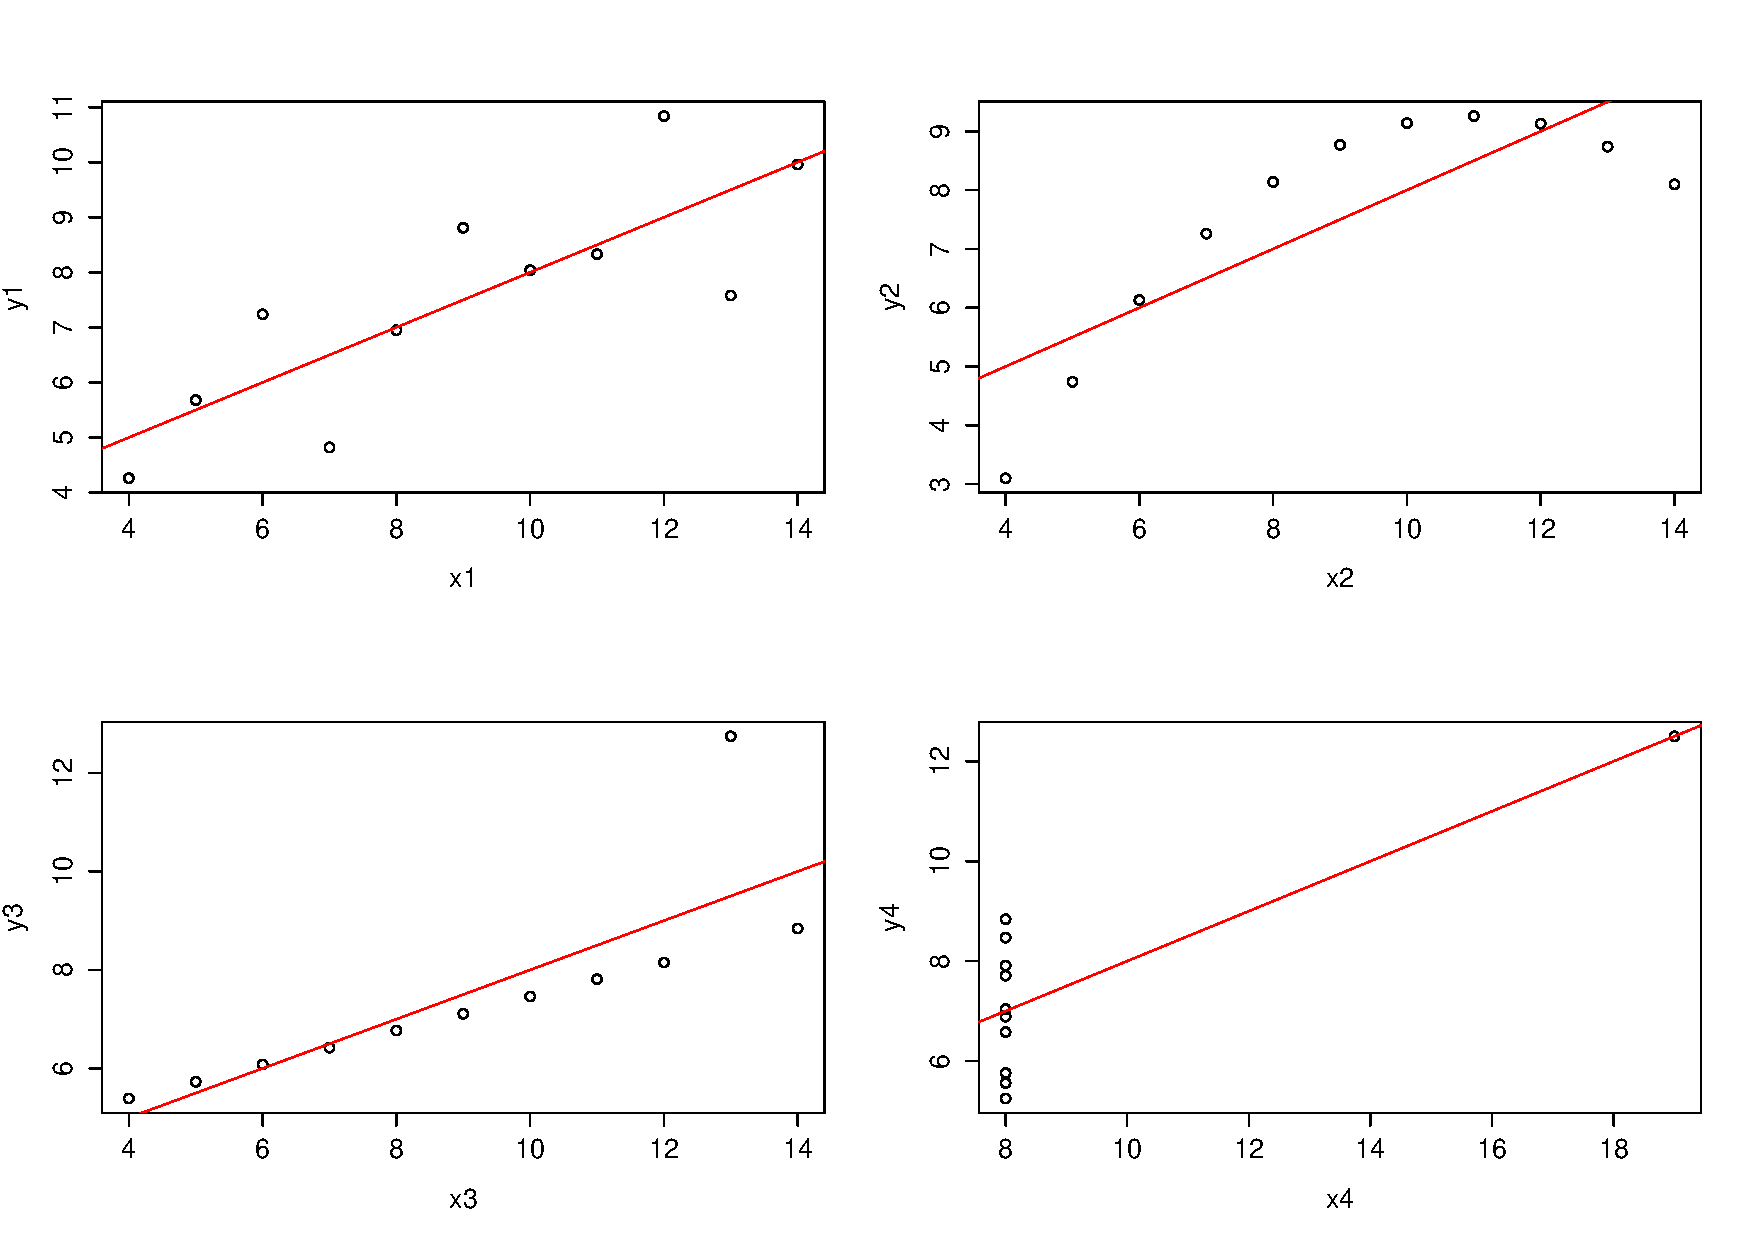
\includegraphics[width=\linewidth]{mateix_r2.pdf}
\end{center}

\end{frame}


\subsection{Intervals de confiança}

\begin{frame}
\frametitle{Supòsits del model}

Suposam d'ara endavant que \emph{cada $E_{x_i}$ segueix una distribució normal amb mitjana $\mu_{E_{x_i}}=0$, la mateixa variància $\sigma_E^2$, i $\sigma(E_{x_i},E_{x_j})=0$ per a cada parella $i,j$}
\bigskip

Si només tenim molt pocs $y$ per a cada $x$, això no es pot contrastar, però implica que els $(e_i)_{i=1,\ldots,n}$ provenen d'una $N(0,\sigma_E^2)$, amb $\sigma_E^2$ estimada per $S^2$, i això sí que ho podem contrastar
\end{frame}

\begin{frame}[fragile]
\frametitle{Exemple 1}
A l'exemple de les alçades i les edats
\begin{verbatim}
> x=c(1,3,5,7,9,11,13)
> y=c(75,92,108,121,130,142,155)
> y.cap=72.321+6.464*x
> errors=y-y.cap
> SSE=sum(errors^2)
> S2=SSE/5
> ks.test(errors,"pnorm",0,sqrt(S2))
	One-sample Kolmogorov-Smirnov test
data:  errors
D = 0.1746, p-value = 0.9583
alternative hypothesis: two-sided
\end{verbatim}
\end{frame}

\begin{frame}[fragile]
\frametitle{Exemple 2}
A l'exemple de la sal i la tensió
\begin{verbatim}
> sal=c(1.8,2.2,3.5,4,4.3,5)
> ten=c(100,98,110,110,112,120)
> ten.cap=86.371+6.335*sal
> errors=ten-ten.cap
> SSE=sum(errors^2)
> S2=SSE/4
> ks.test(errors,"pnorm",0,sqrt(S2))
	One-sample Kolmogorov-Smirnov test
data:  errors
D = 0.2553, p-value = 0.7479
alternative hypothesis: two-sided
\end{verbatim}
\end{frame}

\begin{frame}
\frametitle{Intervals de confiança}
\begin{teorema}
Sota aquestes hipòtesis,
\begin{itemize}
\item Els errors estàndard dels estimadors $b_1$ i $b_0$ són, respectivament,
$$
\frac{\sigma_E}{s_x\sqrt{n}}\quad\mbox{ i }\quad \frac{\sigma_E\sqrt{s_x^2+\overline{x}^2}}{s_x\sqrt{n}}
$$
\end{itemize}
\end{teorema}
\medskip

En aquests errors estàndard (i tots els que segueixen), estimam $\sigma_E$ per mitjà de $S=\sqrt{S^2}$

\end{frame}


\begin{frame}
\frametitle{Intervals de confiança}
\begin{teorema}
Sota aquestes hipòtesis,
\begin{itemize}
\item Les fraccions
$$
\frac{b_1-\beta_1}{\frac{S}{s_x\sqrt{n}}}\quad\mbox{ i }\quad
\frac{b_0-\beta_0}{\frac{S\sqrt{s_x^2+\overline{x}^2}}{s_x\sqrt{n}}}
$$
segueixen lleis $t$ de Student amb $n-2$ graus de llibertat.
\end{itemize}
\end{teorema}

\end{frame}


\begin{frame}
\frametitle{Intervals de confiança}
\vspace*{-2ex}

Per tant, sota aquestes hipòtesis,
\begin{itemize}
\item Un interval de confiança del $(1-\alpha)\cdot 100\%$ per $\beta_1$ és
$$
\left] b_1-t_{n-2,1-\frac{\alpha}{2}} \frac{S}{s_x\sqrt{n}}, b_1+t_{n-2,1-\frac{\alpha}{2}} \frac{S}{s_x\sqrt{n}}\right[
$$
Ho escriurem
$$
\beta_1=b_1\pm t_{n-2,1-\frac{\alpha}{2}} \frac{S}{s_x\sqrt{n}}
$$





\item Un interval de confiança del $(1-\alpha)\cdot 100\%$ per $\beta_0$ és
$$
\beta_0=b_0\pm t_{n-2,1-\frac{\alpha}{2}}\frac{S\sqrt{s_x^2+\overline{x}^2}}{s_x\sqrt{n}}
$$
\end{itemize}

\end{frame}

\begin{frame}
\frametitle{Exemple 1}
\vspace*{-2ex}

A l'exemple de les alçades en funció de l'edat, havíem obtingut la recta
$$
\widehat{y}=72.321+6.464x
$$
i $\overline{x}=7$, $s_x^2=16$, $n=7$, $S^2=8.314$
\medskip

Un interval de confiança al 95\% per $\beta_1$ és
$$
\begin{array}{l}
\displaystyle \beta_1=b_1\pm t_{n-2,1-\frac{\alpha}{2}} \frac{S}{s_x\sqrt{n}}
\\[2ex]
\displaystyle\hphantom{\beta_1} =6.464\pm t_{5,0.975} \frac{\sqrt{8.314}}{4\sqrt{7}}\\[2ex]
\hphantom{\beta_1} =
6.464\pm 2.5706 \cdot 0.2724=6.464\pm  0.7
\end{array}
$$
És l'interval $]5.764,7.164[$
\end{frame}

\begin{frame}
\frametitle{Exemple 1}
\vspace*{-2ex}

A l'exemple de les alçades en funció de l'edat, havíem obtingut la recta
$$
\widehat{y}=72.321+6.464x
$$
i $\overline{x}=7$, $s_x^2=16$, $n=7$, $S^2=8.314$
\medskip

Un interval de confiança al 95\% per $\beta_0$ és
$$
\begin{array}{l}
\displaystyle \beta_0=b_0\pm t_{n-2,1-\frac{\alpha}{2}}\frac{S\sqrt{s_x^2+\overline{x}^2}}{s_x\sqrt{n}}
\\[2ex]
\displaystyle\hphantom{\beta_0}=72.321\pm t_{5,0.975} \frac{\sqrt{8.314}\cdot\sqrt{16+7^2}}{4\sqrt{7}}\\[2ex]
\hphantom{\beta_0} =
72.321\pm 2.5706 \cdot 2.1966=72.321\pm 5.647
\end{array}
$$
És l'interval $]66.674,77.968[$

\end{frame}






\begin{frame}[fragile]
\frametitle{Exemple 1}
\vspace*{-2ex}

Obtenim
\begin{itemize}
\item Interval del 95\% per a $\beta_1$: $]5.764,7.164[$
\medskip

\item Interval del 95\% per a $\beta_0$: $]66.674,77.968[$
\end{itemize}
\begin{verbatim}
> confint(lm(y~x),level=0.95)
                2.5 %    97.5 %
(Intercept) 66.674769 77.968088
x            5.763904  7.164668
\end{verbatim}

\end{frame}



\begin{frame}
\frametitle{Exemple 2}


A l'exemple de la tensió en funció de la sal, havíem obtingut la recta
$$
\widehat{y}=86.371+6.335x
$$
i $\overline{x}=3.467$, $s_x^2=1.2856$, $n=6$, $S^2=5.4365$, $t_{4,0.975}=2.7764$
\medskip

L'interval de confiança al 95\% per $\beta_1$ és\pause
$$
\begin{array}{l}
\displaystyle \beta_1=b_1\pm t_{n-2,1-\frac{\alpha}{2}} \frac{S}{s_x\sqrt{n}}
\\[2ex]
\displaystyle\hphantom{\beta_1} =6.335\pm 2.7764 \cdot\frac{\sqrt{5.4365}}{\sqrt{1.2856}\sqrt{6}}\\[2ex]
\hphantom{\beta_1} = 6.335\pm 2.331
\end{array}
$$
És l'interval $]4.004,8.666[$

\end{frame}

\begin{frame}
\frametitle{Exemple 2}
\vspace*{-2ex}

A l'exemple de la tensió en funció de la sal, havíem obtingut la recta
$$
\widehat{y}=86.371+6.335x
$$
i $\overline{x}=3.467$, $s_x^2=1.2856$, $n=6$, $S^2=5.4365$, $t_{4,0.975}=2.7764$
\medskip

L'interval de confiança al 95\% per $\beta_0$ és\pause
$$
\begin{array}{l}
\displaystyle \beta_0=b_0\pm t_{n-2,1-\frac{\alpha}{2}}\frac{S\sqrt{s_x^2+\overline{x}^2}}{s_x\sqrt{n}}
\\[2ex]
\displaystyle\hphantom{\beta_0}=86.371\pm 2.7764\cdot \frac{\sqrt{5.4365}\cdot\sqrt{1.2856+3.467^2}}{\sqrt{1.2856}\sqrt{6}}\\[2ex]
\hphantom{\beta_0} =86.371\pm 8.502
\end{array}
$$
És l'interval $]77.869, 94.873[$

\end{frame}


\begin{frame}[fragile]
\frametitle{Exemple 2}
\vspace*{-2ex}

Obtenim
\begin{itemize}
\item Interval del 95\% per a $\beta_1$:  $]4.004,8.666[$
\medskip

\item Interval del 95\% per a $\beta_0$:   $]77.869, 94.873[$
\end{itemize}
\begin{verbatim}
> confint(lm(ten~sal),level=0.95)
                2.5 %    97.5 %
(Intercept) 77.869064 94.872509
sal          4.004434  8.666266
\end{verbatim}

\end{frame}



\begin{frame}
\frametitle{Intervals de confiança}
\begin{teorema}
Sota aquestes hipòtesis, i si $x_0$ és un possible valor de $X$
\begin{itemize}
\item L'error estàndard de $\widehat{y}_0$ com a estimador de $\mu_{Y|x_0}$ és
$$
\sigma_E\sqrt{\frac{1}{n}+\frac{(x_0-\overline{x})^2}{ns^2_x}}
$$

\item La fracció
$$
\frac{\widehat{y}_0-\mu_{Y/x_0}}{S\sqrt{\frac{1}{n}+\frac{(x_0-\overline{x})^2}{n
s^2_x}}}$$
segueix una llei $t$ de Student amb $n-2$ graus de llibertat.
\end{itemize}
\end{teorema}
\end{frame}


\begin{frame}
\frametitle{Intervals de confiança}
\begin{teorema}
Sota aquestes hipòtesis, i si $x_0$ és un possible valor de $X$
\begin{itemize}
\item L'error estàndard de $\widehat{y}_0$ com a estimador de $y_0$ és
$$
\sigma_E\sqrt{1+\frac{1}{n}+\frac{(x_0-\overline{x})^2}{ns^2_x}}
$$

\item La fracció
$$
\frac{\widehat{y}_0-y_0}{S\sqrt{1+\frac{1}{n}+\frac{(x_0-\overline{x})^2}{n
s^2_x}}}
$$
segueix una llei $t$ de Student amb $n-2$ graus de llibertat.
\end{itemize}
\end{teorema}
\end{frame}





\begin{frame}
\frametitle{Intervals de confiança}
Per tant, sota aquestes hipòtesis,
\begin{itemize}
\item Un interval de confiança del $(1-\alpha)\cdot 100\%$ per $\mu_{Y|x_0}$ és
$$
\mu_{Y|x_0}=\widehat{y}_0\pm t_{n-2,1-\frac{\alpha}{2}} S\sqrt{\frac{1}{n}+\frac{(x_0-\overline{x})^2}{n
s^2_x}}
$$

\item Un interval de confiança del $(1-\alpha)\cdot 100\%$ per $y_0$ és
$$
y_0=\widehat{y}_0\pm t_{n-2,1-\frac{\alpha}{2}} S\sqrt{1+\frac{1}{n}+\frac{(x_0-\overline{x})^2}{n
s^2_x}}
$$
\end{itemize}

\end{frame}



\begin{frame}
\frametitle{Exemple 1}
\vspace*{-2ex}

A l'exemple de les alçades en funció de l'edat, havíem obtingut la recta
$$
\widehat{y}=72.321+6.464x
$$
i $\overline{x}=7$, $s_x^2=16$, $n=7$, $S^2=8.314$
\medskip

Suposem que volem estimar l'alçada $y_0$ d'un nin de $x_0=10$ anys  
$$
\widehat{y}_0=72.321+6.464\cdot 10=136.961
$$

Interval de confiança al 95\% per aquest valor? Interval de confiança al 95\% per al valor esperat?
\end{frame}



\begin{frame}
\frametitle{Exemple 1}
\vspace*{-2ex}


Un interval de confiança al 95\% per $y_0$ és
$$
\begin{array}{l}
\displaystyle
y_0=\widehat{y}_0\pm t_{n-2,1-\frac{\alpha}{2}} S\sqrt{1+\frac{1}{n}+\frac{(x_0-\overline{x})^2}{ns^2_x}}
\\[2ex]
\displaystyle\hphantom{y_0}=136.961\pm t_{5,0.975} \sqrt{8.314}\cdot\sqrt{1+\frac{1}{7}+\frac{(10-7)^2}{7\cdot 16 }}\\[2ex]
\hphantom{y_0} =
136.961\pm 2.5706 \cdot  3.189=136.961\pm  8.198
\end{array}
$$
És l'interval $]128.8,145.2[$

\end{frame}


\begin{frame}
\frametitle{Exemple 1}
\vspace*{-2ex}


Un interval de confiança al 95\% per $\mu_{Y|x_0}$ és
$$
\begin{array}{l}
\displaystyle
\mu_{Y|x_0}=\widehat{y}_0\pm t_{n-2,1-\frac{\alpha}{2}} S\sqrt{\frac{1}{n}+\frac{(x_0-\overline{x})^2}{ns^2_x}}
\\[2ex]
\displaystyle\hphantom{y_0}=136.961\pm t_{5,0.975} \sqrt{8.314}\cdot\sqrt{\frac{1}{7}+\frac{(10-7)^2}{7\cdot 16 }}\\[2ex]
\hphantom{y_0} =
136.961\pm 2.5706 \cdot  1.362=136.961\pm  3.501
\end{array}
$$
És l'interval $]133.5, 140.5[$

\end{frame}


\begin{frame}[fragile]
\frametitle{Exemple 1}
\vspace*{-2ex}

\begin{verbatim}
> newdata=data.frame(x=10)
> predict.lm(lm(y~x),newdata,
  interval="prediction",level=0.95)
       fit      lwr     upr
1 136.9643 128.7665 145.162
> predict(lm(y~x),newdata,
  interval="confidence",level=0.95)
       fit      lwr      upr
1 136.9643 133.4624 140.4662
\end{verbatim}



\end{frame}

\begin{frame}
\frametitle{Té sentit una regressió lineal?}

Si $\beta_1=0$,  el model de regressió lineal no té sentit:
$$
Y=\beta_0+E
$$
i les variacions en els valors de $Y$ són totes degudes a l'error.
\medskip

El contrast
$$
\left\{\begin{array}{l}
H_0:\beta_1=0\\
H_1:\beta_1 \neq 0
\end{array}
\right.
$$
el podem realitzar amb l'interval de confiança per a $\beta_1$: si 0 no hi pertany, 
rebutjam la hipòtesi nu\l.la
\end{frame}


\begin{frame}
\frametitle{Exemples}
\vspace*{-2ex}

Hem obtingut:
\begin{itemize}
\item A l'exemple 1, un interval del 95\% per a $\beta_1$ és $]5.764,7.164[$
\medskip

\item A l'exemple 2, un interval del 95\% per a $\beta_1$:  $]4.004,8.666[$
\end{itemize}
\medskip

Als dos casos concloem que $\beta_1\neq 0$ i que per tant tenia sentit fer la regressió lineal
\end{frame}

\begin{frame}[fragile]
\frametitle{Amb R}
{\footnotesize \begin{verbatim}
> summary(lm(alçada~edat))
...
Coefficients:
            Estimate Std. Error t value Pr(>|t|)    
(Intercept)  72.3214     2.1966   32.92 4.86e-07 ***
edat          6.4643     0.2725   23.73 2.48e-06 ***
---
Signif. codes:  0 ‘***’ 0.001 ‘**’ 0.01 ‘*’ 0.05
   ‘.’ 0.1 ‘ ’ 1 
...
\end{verbatim}
}

Els \red{\texttt{t value}} són els dels contrastos amb $H_0:$ ``coeficient $=0$'', i els p-valors són els d'aquests
 contrastos. Podem rebutjar que $\beta_1=0$ (i que $\beta_0=0$)

\end{frame}

\end{document}
